\chapter{High Voltage System}
\label{ch:fdsp-hv}

%%%%%%%%%%%%%%%%%%%%%%%%%%%%%%%%%%%%%%%%%%%%%%%%%%%%%%%%%%%%%%%%%%%%
\section{High Voltage System (HV) Overview}
\label{sec:fdsp-hv-ov}


%%%%%%%%%%%%%%%%%%%%%%%%%%%%%%%%%
\subsection{Introduction}
\label{sec:fdsp-hv-intro}
A liquid argon cryostat requires an equipotential cathode plane of high voltage (CPA-plane), and a precisely regulated interior electric field to drive electrons from particle interactions to the sensor planes (APA's, see volume 3A). This requires planar components (CPA's)  held at high voltage, and formed sets of conductors at graded voltages on the top and bottom (FC's) and sides (EW-FC's) of the central drift volume. After a discussion of the materials used in construction, this document will discuss the CPA-plane first, followed by the field shaping components. 




The operating principle is illustrated in Figure~\ref{figure-label}... (add figure)

\begin{dunefigure}[One unit of DUNE showing CPA's,  and APA's]{fig:HV_Module}
{One unit of DUNE showing CPA's and APA's (Credit: CAD model)}
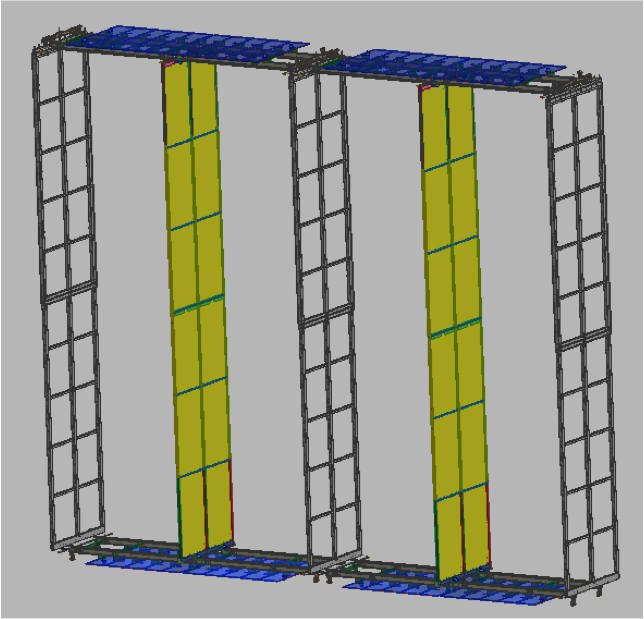
\includegraphics[width=0.8\textwidth]{HV_Module.png}
\end{dunefigure}

%%%%%%%%%%%%%%%%%%%%%%%%%%%%%%%%%%%%%
\subsection{Design Considerations}
\label{sec:fdsp-hv-des-consid}
This section contains best practices and requirements, as well as interferences and experience from ProtoDune. A discussion of MONITORING REQUIREMENTS will also come here.

%%%%%  Design to identify MIPs -- wire pitch and other params
 
...

\fixme{Anne suggests: Within this section add ref to requirements document  when it's ready, and maybe list the most important half dozen in a table here). E.g.,}  

\begin{dunetable}
[HV System Requirements]
{p{0.35\linewidth}p{0.62\linewidth}}
{tab:hvphysicsreqs}
{HV System Requirements}   
 Requirement & Physics Requirement Driver \\ \toprowrule
Exceed minimum electric field in TPC drift volume & Maintain adequate particle ID, which is impacted by slower drift speed and increased diffusion and space charge effects. \\ \colhline
  Do not exceed maximum electric field in LAr volume & Avoid damage to detector to enable data collection over long periods. \\ \colhline
 Minimize power supply ripple & Keep readout electronics free from external noise, which confuses event reconstruction. \\ \colhline
 Maximize power supply stability & Maintain the ability to reconstruct data taken over long period.  Maintain high operational uptime to maximize experimental statistics. \\ \colhline
 Provide adequate decay constant for discharge of the cathode surface and field cage  & Avoid damage to detector to enable data collection over long periods. Maintain high operational uptime to maximize experimental statistics. \\ \colhline
 Provide redundancy in all HV connections & Avoid single point failures in detector which interrupt datataking.\\ 
\end{dunetable}

\fixme{By the end of the volume, for every requirement listed in this section, there should exist an explanation of how it will be satisfied.}


%%%%%%%%%%%%%%%%%%%%%%%%%%%%%%%%
\subsection{Scope (Rob)}
\label{sec:fdsp-hv-scope}

This section discusses the  scope of the HV system, which includes the continued procurement of materials for, and the fabrication, testing, delivery and installation of systems to generate, distribute, and regulate voltages which create a precision electric field within the DUNE detector volume. 

The HV system consists of components both exterior and interior to the cryostat. The HV power supplies and filters pass through the HV feedthrough and are further distributed by components which form part of the TPC structure. These are:
\begin{itemize}
\item Power Supply
\item Cathode Plane
\item Top and Bottom Field Cages and Ground Planes
\item Endwall Field Cages 
\end{itemize}
The TPC has a 2 central Cathode Plane Arrays (CPA-arrays), 57.5m long and 12m tall, with two symmetric drift volumes on both sides. There are 25 CPA-planes in each CPA-array, installed contiguously along the length of the TPC. A CPA-plane is assembled from 2 side-by-side Cathode Plane Assembly Panel (CPA-panels). Each CPA-panel is 1.2m in width and 12m tall, formed from 6 vertically stacked modules, and supported from above by the CPA installation rail, through a single link.
A CPA consists of a FR4 frame that encloses and supports the resistive panels (modules).  Each CPA is approximately 1.1m wide and 6m long and is constructed from three modules.  Six CPA's together form the CPA plane. 
The sides of the drift volumes on both sides of the CPA-plane are covered by the FC and EW field cage modules to define a uniform drift field of 500V/cm, which decreases gradually over 3.6m from the high voltage CPA (-180kV) to ground potential at the APA sensor planes, . The cathode bias is provided by an external high voltage power supply through an HV feedthrough connecting to the CPA-plane inside the cryostat.
The Field Cage modules have two distinctive types: the top/bottom (FC), which run the full length of the detector, and the end walls (EW's), which complete the detector at either end. The modules of both systems are constructed from an array of roll-formed aluminum open profiles supported by FRP (fiber reinforced plastic) structural beams. A resistive divider chain interconnects all the metal profiles to provide a linear voltage gradient between the cathode and anode planes.  The top/bottom modules are nominally 2.3m wide by 3.6m long. 

A ground plane of tiled perforated stainless steel sheet panels is mounted on the outside surface of each of the top/bottom field cage modules with a 20cm clearance. The top and bottom  FC modules are supported by the CPAs and APAs. The end wall modules are 1.5m tall by 3.6m long. They are stacked 4 units high to cover the 6m height of the TPC.  These EW-FC modules are supported by the installation rails above  the APAs and CPAs, which are part of the Detector Support Structure (DSS). 




%%%%%%%%%%%%%%%%%%%%%%%%%%%%%%%%%%%%%%%%%%%%%%%%%%%%%%%%%%%%%%%%%%%%
\section{HV System Design}
\label{sec:fdsp-hv-design}

\subsection {High Voltage Power Supply and Feedthrough (Sarah)}
The HV delivery system consists of
\begin{itemize}
\item A power supply (or multiple).
\item HV cables.
\item Filter resistors.
\item And HV feedthroughs.
\end{itemize}

There are two options being considered for high voltage delivery.  In one option, each cathode would have its own power supply.  In an alternate plan, one power supply would supply the voltage to two feedthroughs via a splitter.

The planned power supply model is a Heinzinger PNChp 200000 with a maximum output voltage of \SI{200}{kV} and a maximum current draw of \SI{0.5}{mA}.  An additional option is an existing \SI{300}{kV} \SI{0.5}{mA} model. 

The high voltage cables will be either Dielectric Sciences model number 2134 capable of \SI{200}{kV} DC or 2236 capable of \SI{320}{kV} DC.  

The filter resistors will be placed in between the power supply and the feedthrough.  Along with the cables, they reduce the discharge impact by partitioning the stored energy in the system.  The resistor-cable assembly also serves as a low-pass filter reducing the $\sim$\SI{30}{kHz} voltage ripple on the output of the power supply.

The targeted noise values set the upper limit of residual voltage ripple on the cathode to be \SI{0.5}{mV}\todo{I made this up}.  The Heinzinger 300000 model specifies the ripple to be less than or equal to $0.001\%V_{nom} \pm 50$ mV.  Assuming cable lengths of \SI{100}{ft} and \SI{10}{ft} between the filters, and between the filter and feedthrough, the noise reduction can be attained with resistances as low as a M$\Omega$. 

The current plan for the filters is a cylindrical design.  Here, a high voltage resistor will be electrically connected on each end to a cable receptacle.  The resistor should be selected to withstand a large over-power condition.  Radially out from the resistor is an insulator.  In other designs, this has been transformer oil or UHMW PE.  The outer case of the filter is a grounded stainless-steel shell.

The high voltage feedthrough is planned to be based on the successful ICARUS design.  The voltage is transmitted by a stainless steel center conductor.  On the warm side of the cryostat, this conductor mates with a cable end.  Inside the cryostat, the end of the center conductor has a spring-loaded tip that will contact a receptacle cup mounted on the cathode delivering high voltage to the field cage.  The center conductor of the feedthrough is surrounded by UHMW PE.  The upper bound of operating voltage on a feedthrough is, to first order, set by the maximum electric field on the feedthrough.  This electric field is reduced by increasing the insulator radius.  For the target voltage, the feedthrough will use a UHMW PE cylinder of roughly 6'' diameter.  In the gas space and into at least 6'' of the liquid, the insulator will be surrounded by a tight fitting stainless steel ground tube.  The ground tube will have a 10'' Conflat flange welded on for attachment to the cryostat.

\subsection{CPA (Vic, Steve)}
The CPA provides a constant potential surface at -180 kV for the DUNE SP TPC.  It receives its high voltage from the HV Feedthrough which makes contact with the HV Bus mounted on the CPA frame.  It also provides HV to the first profile on the Top and Bottom Field Cage (FC) elements and to the EndWall FCs as well.  The constant potential surface is a resistive panel (RP) comprised of a thin layer of carbon-impregnated kapton laminated to both sides of a 3 mm thick FR4 sheet of 1.2 m X 2 m size.  The surface resistivity of the RPs is required to be in the range of 1-10 MOhms/square in order to provide for slow reduction of accumulated charge in the event of a discharge.  Other HV components of the CPA include field shaping strips (FSSs) mounted to the CPA frames, aluminum profiles to form the first elements of the field cage, and cable segments forming the HV Bus.  The CPA frames are required to support in addition to the HV components, Top and Bottom FC units attached to both sides of the CPA panel.  Care must be taken to ensure that no sharp points or edges are present on any of the resistive and/or conductor materials.  
\subsection{Field Cages}

\subsection{General Considerations}

A uniform electric field is required to drift ionization electrons towards the APAs. Field cages consisting of equidistant resistive strips form a barrel 
around the active drift volume. The resistive strips are biased at different potential to establish a uniform field inside the LAr volume.
For the DUNE far detector we plan to use extruded aluminum profiles as a cost effective way to establish the equipotential surfaces. 

The shape of resistive strips is critical as it determines the strength of the electric field between a given profile and its neighboring profiles as well as
other surrounding parts, including the stainless steel membrane which is electrically at ground level. Electric fields need to be well below 30kV/cm 
to enable safe TPC operation.

The identified profile (Dahlstrom Roll Form, \#1071) is estimated to lead to E fields of up to 12~kV/cm under the assumption of DUNE field cage configuration 
and operating voltage. Figure \ref{fig:Profile-Efield} illustrates results from a E field calculation.

\begin{dunefigure}
[Electric field map (color) and equipotential contours of an array of roll formed profiles biased up to -180kV and a ground clearance of 20cm]{fig:Profile-Efield}
{Electric field map (color) and equipotential contours of an array of roll formed profiles biased up to -180kV and a ground clearance of 20cm(Credit: CAD model)} 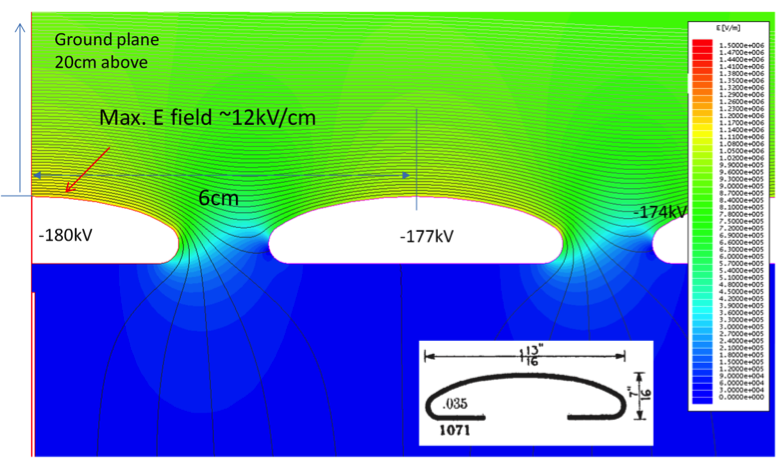
\includegraphics[width=0.8\textwidth]{Profile-Efield.png}
\end{dunefigure}

The profiles ends are equipped with UHMW polyethylene caps to reduce the risk of arc formation.  These caps are designed to have sufficient wall thickness (6mm) to withstand the full voltage across their walls.

The Aluminum profiles are attached to fiber-reinforced plastic (FRP) pultruded structural elements, including I-beams and box beams.  
Pultruded FRP material is non-conductive and strong enough to withstand the loads of field cage in the temperature range of -150C and 23C.
%FRP has all of the reinforcing fibers running along the main axis of the section being used.  
The FRP material will meet the International Building Code classification for flame spread and smoke development of a Class A, as characterized by ASTM E84.  


The field cage modules have two distinctive styles: the top/bottom (T/B), and the end wall both of which are described below. 
A resistive divider chain interconnects all the Aluminum profiles to provide a linear voltage gradient between the cathode and anode planes.  The T/B modules are nominally 2.3m wide by 3.6m long. A ground plane in the form of tiled perforated stainless steel sheet panels is mounted on the outside surface of the T/B field cage module with a 20cm clearance. The T/B modules are supported by the CPAs and APAs. The end wall modules are 1.5m tall by 3.6m long. They are stacked 8 units high to cover the 12m height of the TPC.  These modules are supported by the installation rails above the APAs and CPAs.   


\subsubsection{Top and Bottom field cages (Mike)}
Discussion of Top and Bottom field cages comes here.
\subsubsection{ Endwall field cages (Thomas)}

The End Wall Field Cage (EWFC) for each drift volume consists of two endwalls (EW), one on each side of the drift volume. Each endwall is in turn composed of 8 FC endwall modules. 

There are two different types of EW modules and each of these comes in a regular and in a mirrored configuration to account for 
mounting constraints and to match the detector geometry. Figures \ref{fig:FCendwall_top} and \ref{fig:FCendwall_panel} illustrate the layout for the topmost 
and the baseline panels, respectively.

\begin{dunefigure}[Uppermost panel of the field cage endwall.]{fig:FCendwall_top}{Uppermost panel of the field cage endwall. {\color{red} NOTE: need to replace figure with updated version for DUNE, e.g. without middle FRP cross member.}}
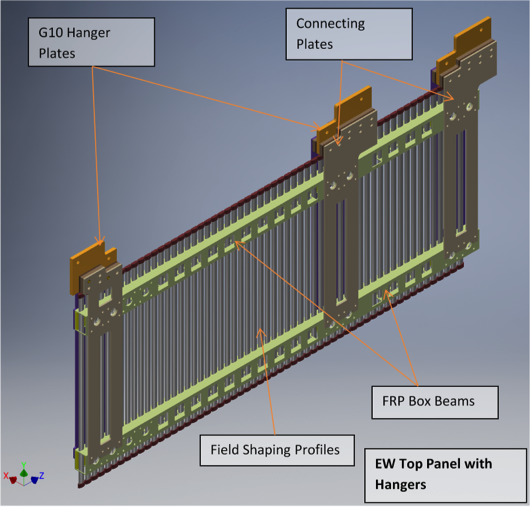
\includegraphics[width=0.48\textwidth]
{FCendwall_top-panel.png}
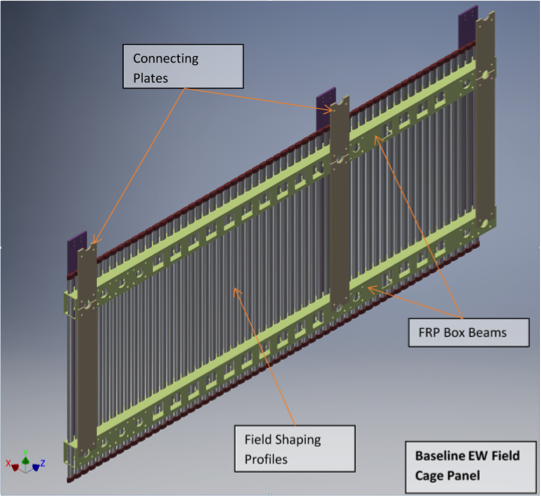
\includegraphics[width=0.48\textwidth]{FCendwall_panel.png}
\end{dunefigure}

Each EWFC module consists of two FRP box beams which are 3.6 m long. The box beam design also incorporates cutouts on the outside face to minimize charge build up. Box beams are connected using $1/2$\"Ó thick FRP plates. The plates are connected to the box beams using a shear pin and bolt arrangement. The inside plates facing the active volume are connected using special stainless steel slip nuts and stainless steel bolts. The field shaping profiles are connected to the top box beam using stainless steel slip nuts, an FRP angle, and two screws each. The profiles are connected to the bottom box beam with a slip nut that is held in place by friction.

\begin{dunefigure}[Baseline field cage panel.]{fig:FCendwall_panel}{Baseline field cage panel. {\color{red}NOTE: need to replace figure with updated version for DUNE, e.g. without middle FRP cross member.}}
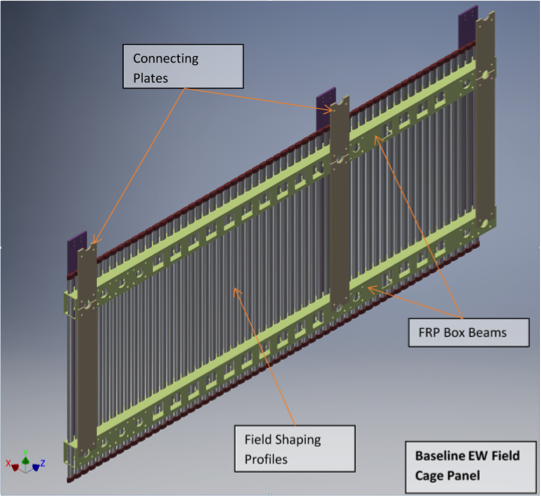
\includegraphics[width=0.48\textwidth]{FCendwall_panel.png}
\end{dunefigure}

%\begin{center}
%   \parbox[t]{0.47\textwidth}{
 %  \resizebox{0.47\textwidth}{!}{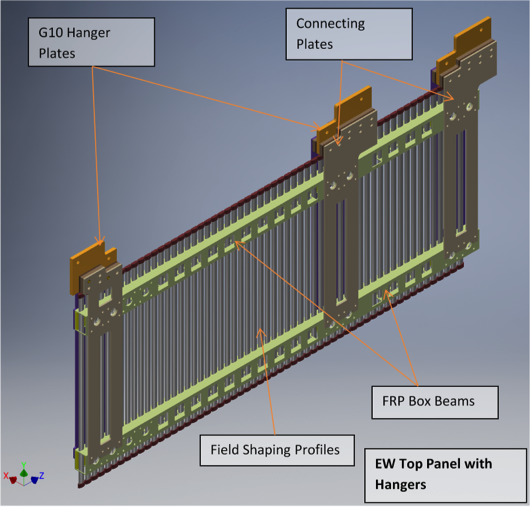
\includegraphics[width=0.48\textwidth]{FCendwall_top-panel.png}}
%\caption{\label{fig:FCendwall_top} Uppermost panel of the field cage endwall. {\color{red} NOTE: need to replace figure with updated version for DUNE, e.g. without middle FRP cross member.}}}
%\makebox[0.025\textwidth]{}
 %  \parbox[t]{0.48\textwidth}{
 %  \resizebox{.48\textwidth}{!}{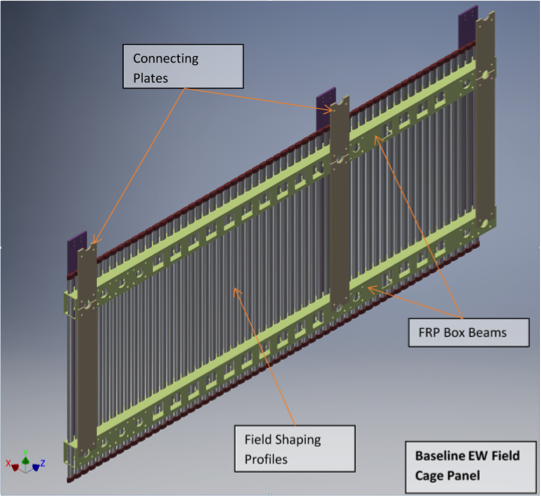
\includegraphics[width=0.48\textwidth]{FCendwall_panel.png}}
%\caption{\label{fig:FCendwall_panel} Baseline field cage panel. {\color{red}NOTE: need to replace figure with updated version for DUNE, e.g. without middle FRP cross member.}}}
%\end{center}




\subsection{Electrical Interconnections (Glenn)}


%%%%%%%%%%%%%%%%%%%%%%%%%%%%%%%%%%%
\subsection{Quality Assurance}
\label{sec:fdsp-hv-qa}

\fixme{Include an image of the subsystem, indicating its parts. Show how the system fits into the overall system).}


%%%%%%%%%%%%%%%%%%%%%%%%%%%%%%%%%%%%%%%%%%%%%%%%%%%%%%%%%%%%%%%%%%%%
\section{Production and Assembly}
\label{sec:fdsp-hv-prod-assy}

%%%%%%%%%%%%%%%%%%%%%%%%%%%%%%%%%%
\subsection{Power Supplies and Feedthroughs}
\label{sec:fdsp-hv-supplies-feedthroughs}

Discussion of parts procurement, assembly, and testing.

Additional power supplies can be bought through Heinzinger. \todo{Do we have access to the PD units?}  The high voltage cable can be bought through Dielectric Sciences.  

The power supply will be tested extensively along with the controls and monitoring software.  Features to be included in the software are:
\begin{itemize}
\item The ability to ramp, or change the voltage.  The rate and an ability to pause the ramp shall be included.
\item An input for a user-defined current limit.  This parameter is the current value at which the supply reduces the voltage output to stay below the current limit.  The current limiting is done in hardware.
\item An input for a trip threshold.  At this current reading, the program would reduce the voltage output through software.  In previous experiments, the trip function in software would set the output to \SI{0}{kV}.
\end{itemize}
\noindent Additionally, the software should record the current and voltage read back values with a user-defined frequency, and also any irregular current or voltage events.

The high voltage feedthroughs, filters, and splitter are custom devices.  One feedthrough option is to use the ProtoDUmNE-SP design and order an additional unit from Cinel.  High voltage splitters are already on hand if they are desired.

%%%%%%%%%%%%%%%%%%%%%%%%%%%%%%%%%%
\subsection{CPA}
\label{sec:fdsp-hv-supplies}

The component parts of the CPA assembly will be produced by commercial vendors for the following items:
\begin{itemize}
\item Manufactured FR4 RP frames packed into 3 RP Unit kits making up a CPA Panel
\item Carbon-impregnated Kapton coated resistive panels (RPs) and Field Shaping Strips (FSSs)
\item HV cable segments and wire jumpers making up the CPA HV Bus and RP interconnects
\item Machined Brass tabs for connecting RPs, HV Bus, and FSSs
\item Top, Bottom, and exterior edge profiles
\end{itemize}
The above items will be packaged into CPA Panel kits by the vendors and will be sent to the assembly factories.  The basic construction unit for an assembly factory will be a pair of CPA Panels so that shipment to SURF from an assembly factory will consist of two CPA Panels that are paired on site to form a CPA Plane.

The basic element of the CPA is a RP mounted in a machined slot in the top, bottom and sides of FR4 frames.  There are three different types of these elements - an Upper which has as its top frame the CPA mounting bracket and Top FC hinge, a Middle, and a Lower which has as its bottom frame a Bottom FC hinge.  Two such RP elements are bolted together and pinned to form a shipment Unit of size 1.2 m X 4 m.  These Units are assembled horizontally on a smooth, flat table to meet the dimensional requirements of CPA construction.  In addition to the frames and RPs, FSSs are mounted on the exposed sides of the FR4 frames, aluminum profiles are attached to the top and bottom of the Upper and Lower elements, and cables are attached to the RPs to form segments of the HV Bus.  The shipment Unit comes in 3 varieties in order to make a full 12 m tall CPA Panel.  These are : 1) an Upper element attached to a Middle element, 2) two Middle elements connected, and 3) a Middle element attached to a Lower element.  The Unit order in the shipping crate from bottom to top is Upper/Middle, Middle/Middle, Middle/Lower.  For the 10 kt DUNE SP TPC, there are 100 Upper elements, 100 Lower elements and 400 Middle elements which make up the 100 CPA Panels of the TPC.

Upon arriving at the DUNE site, The shipping crate is unpacked with the Middle/Lower Unit placed in a vertical stand on the floor of the ``toaster'' region.  Next, the Middle/Middle Unit is removed and vertically attached to the Middle Lower Unit.  Finally, the Upper/Middle unit is removed and attached.  This assembly makes up a CPA Panel.  The Panel is lifted and vertically attached to its trolley with a FR4 hangar.

Two CPA Panels are paired to form a Plane which forms the unit for FC attachment.  There are a total of 50 CPA Panel pairs arranged in the DUNE cryostat in two rows of 25 each.  After the Panels are paired, FC units are attached folded against the CPA and the full CPA/FC assembly is placed in the DUNE cryostat through the access door.  Upon deployment of the folded Top and Bottom FC units (and including the EndWalls), the TPC field cage is complete.

It should also be noted that the CPA Panels on each end of the 25 Panel pairs are special - they have mounted on them aluminum profiles along the exterior side to form the first element of the field cage.  They also contain parts of the HV Bus mounted on the CPA frames.  The HV Bus forms a continuous loop from the HV Input through the top of the 25 CPA Panel pairs, down the far external side, back along the bottom and up the  external side back to the HV Input.

\subsection{Field Cages}

%

\subsubsection{Top and Bottom field cages}
Discussion of parts procurement, assembly, and testing.

\subsubsection{Endwall field cages}
Discussion of parts procurement, assembly, and testing.


\subsection{Electrical Interconnections}

Discussion of parts procurement, assembly, and testing.



%%%%%%%%%%%%%%%%%%%%%%%%%%%%%%%%%%%%%%%%%%%%%%%%%%%%%%%%%%%%%%%%%%%%
\section{Interfaces (Bo)}
\label{sec:fdsp-hv-intfc}
%
%\fixme{Include an image of each interface in appropriate section.}
%
\fixme{Editors at meeting of 2/13 have suggested that detailed interface list will go into a separate chapter. Accordingly, I have commented out the subsections. RKP.}
\fixme{Need a brief paragraph calling out the main issues only. RKP}
%
%%%%%%%%%%%%%%%%%%%%%%%%%%%%%%%%%%%
%\subsection{Interfaces to APA}
%\label{sec:fdsp-hv-intfc-cpa-fc}
%
%
%%%%%%%%%%%%%%%%%%%%%%%%%%%%%%%%%%%
%\subsection{Interface to DSS}
%\label{sec:fdsp-hv-intfc-dss}
%
%
%%%%%%%%%%%%%%%%%%%%%%%%%%%%%%%%%%%
%\subsection{Interface to PDS}
%\label{sec:fdsp-hv-intfc-pds}
%
%%%%%%%%%%%%%%%%%%%%%%%%%%%%%%%%%%%
%\subsection{Interface to CE}
%\label{sec:fdsp-hv-intfc-ce}
%
%%%%%%%%%%%%%%%%%%%%%%%%%%%%%%%%%%%
%\subsection{Interface to Calibration}
%\label{sec:fdsp-hv-intfc-cal}
%
%
%
%%%%%%%%%%%%%%%%%%%%%%%%%%%%%%%%%%%%%%%%%%%%%%%%%%%%%%%%%%%%%%%%%%%%
\section{Installation, Integration and Commissioning}
\label{sec:fdsp-hv-install}

%%%%%%%%%%%%%%%%%%%%%%%%%%%%%%%%%%%%
\subsection{Transport and Handling}
\label{sec:fdsp-hv-install-transport}

The power supply, cables, filters, and feedthroughs will be sent to site in standard shipping crates.  Handlers will wear gloves when handling insulators that will be between high voltage and ground.  Surfaces can be cleaned with alcohol and allowed to dry.

CPA Panels will be shipped in crates to the SURF site.  The 12 m Panels will be disassembled into their three RP Units, loaded into the crates with all hardware needed to complete the Panel assembly at the SURF site.  Each shipment should consist of two crates which contain the two Panels that will be paired to form a CPA Plane.  There will be very little room for storage at the SURF site, so it is important to ship Panels in this way so that final assembly, integration, and installation can proceed as soon as components are received.

%%%%%%%%%%%%%%%%%%%%%%%%%%%%%%%%%%%
\subsection{Integration }
\label{sec:fdsp-hv-install-pds-elec}

%%%%%%%%%%%%%%%%%%%%%%%%%%%%%%%%%%%%%%%%%%%%%%%%%%%%%%%%%%%%%%%%%%%%
\section{Quality Control}
There will be excellent quality control, based on documented assembly, testing, transport, and installation procedures.
\label{sec:fdsp-hv-qc}

Power supplies used in the DUNE will be tested before installation.  Output voltages and currents must be checked on a known load. 

The feedthrough and filters should be tested at the same time preferably with the planned power supply.  The feedthrough must hold the goal \todo{or requirement?} voltage in TPC-quality liquid argon ($\tau\geq$\SI{1.6}{ms}) for at least a day.  The ground tube submersion and electric field environment of the test setup should be comparable to the real field cage setup or more challenging ({\it e.g.}\ the test liquid level can be lower than DUNE's but not higher).  Additionally, the feedthrough must be leak tight to XXXX \todo{The MAWP is pretty low; I don't know if there's a required pressure test.}

CPA QC consists of forms that are filled out as part of the various procedures from initial assembly at factories to the final testing of connections in the DUNE cryostat.  A group of QC forms filled out during initial Panel Unit assembly travels in the shipping crate with the Panel.  At SURF, Panel and Plane assemblies have their own set of QC forms for CPA assembly and for CPA/FC integration.  Finally, before Top and Bottom FC deployment, a final check of all electrical connections on the CPA and between the CPA and the Top, Bottom, and EndWall FCs is completed.  All of these forms are documented and available in the DUNE Document Database.

%%%%%%%%%%%%%%%%%%%%%%%%%%%%%%%%%%%%
\subsection{Protection and Assembly (Local)}
\label{sec:fdsp-hv-qc-local}


%%%%%%%%%%%%%%%%%%%%%%%%%%%%%%%%%%%
\subsection{Post-factory Installation (Remote)}
\label{sec:fdsp-hv-qc-remote}





%%%%%%%%%%%%%%%%%%%%%%%%%%%%%%%%%%%%%%%%%%%%%%%%%%%%%%%%%%%%%%%%%%%%
\section{Safety}

Safety is a the central consideration in the design of the HPS system in all phases including fabrication, installation, and operations. priority for the will be the highest priority at all times. There will be documented assembly, testing, transport, and installation procedures.

\label{sec:fdsp-hv-safety}

%%%%%%%%%%%%%%%%%%%%%%%%%%%%%%%%%%%
% add subsections and labels if needed \subsection{}
%\label{sec:fdsp-hv-safety-}


%%%%%%%%%%%%%%%%%%%%%%%%%%%%%%%%%%
%\subsection{}
%\label{sec:fdsp-hv-safety}



%%%%%%%%%%%%%%%%%%%%%%%%%%%%%%%%%%%%%%%%%%%%%%%%%%%%%%%%%%%%%%%%%%%%
\section{Organization and Management}
\label{sec:fdsp-hv-org}


%%%%%%%%%%%%%%%%%%%%%%%%%%%%%%%%%%%
\subsection{HV System Consortium Organization}
\label{sec:fdsp-hv-org-consortium}

At present, the consortium is gathering together all the institutions that are participating to the design, construction and assembly of the HV systems for both ProtoDUNE SP and DP detectors. There is still the need to expand this list in the near future with effort in including new EU participants.

\begin{dunetable}
[HV Consortium Participants]
{p{0.35\linewidth}p{0.25\linewidth}p{0.35\linewidth}}
{tab:hvconsortiumparticipants}
{HV Consortium Participants}   
 Institution & Investigator & Contact \\ \toprowrule
EU: CERN & Francesco Pietropaolo & francesco.pietropaolo@cern.ch  \\ \colhline
USA: Argonne National Lab   &   Steve Magill   &   srm@anl.gov   \\ \colhline
USA: Brookhaven National Lab  &  Bo Yu  &  yubo@bnl.gov  \\ \colhline
USA: University of California (Berkeley)  & Cheng Ju Lin  &  cjslin@lbl.gov  \\ \colhline
USA: University of California (Davis)  & Emilija Pantic   &   pantic@ucdavis.edu  \\ \colhline
USA: Fermi National Accelerator Lab  & Sarah Lockwitz   &   lockwitz@fnal.gov  \\ \colhline
USA: University of Houston & A. Renshaw   &   arenshaw@central.uh.edu  \\ \colhline
USA: Kansas State University & Glenn Horton-Smith   &   gahs@ksu.edu  \\ \colhline
USA: Lawrence Berkeley National Lab & Cheng Ju Lin   &   cjslin@lbl.gov  \\ \colhline
USA: Louisiana State University & Thomas Kutter   &   kutter@phys.lsu.edu  \\ \colhline
USA: South Dakota School of Mines and Technology  & J. Reichenbacher	&   Juergen.Reichenbacher@sdsmt.edu  \\ \colhline
USA: Stony Brook University  & Micheal Wilking   &   michael.wilking@stonybrook.edu  \\ \colhline
USA: University of Texas (Arlington) & Jaehoon Yu   &   jaehoonyu1@gmail.com  \\ \colhline
USA: Virginia Tech. & Jon Link   &   jmlink@vt.edu  \\ \colhline
USA: College of William and Mary  &  Jeff Nelson   &   jknels@wm.edu  \\

\end{dunetable}
The Consortium has the following Management Structure:
\begin{itemize}
 \item Consortium Leader: Francesco Pietropaolo (CERN)
 \item Technical Leader: Bo Yu (BNL)
 \item TDR/TP Editor: Rob Plunkett (FNAL)
 \item HVS design and integration lead: Vic Guarino (ANL)
\end{itemize}

In the HVS consortium organisation, each institution is naturally assuming the same responsibilities as for the developments of ProtoDUNE. The consortium is organised into working groups addressing the design and  R and D phases and the hardware production and installation.

\begin{itemize}
\item WG1. Design optimization for SP and DP; assembly, system integration, detector simulation, physics requirements for monitoring and calibrations. Conveners: Jeff Nelson, Vic Guarino, Bo Yu
\item WG2. R and D activities, R and D facilities. Conveners: Francesco Pietropaolo, Ting Miao
\item WG3. Single phase-CPA: Procurement, in situ QC, resistive Panels, frame strips, Electrical connections of planes / QC, Assembly, Shipment to assembly site / QC. Conveners: Stephen Magill
\item WG4. DP Cathode. Convener: Jae Yu
\item WG5. Field cage modules. Conveners: Thomas Kutter, Michael Wilking, Jeff Nelson, Jae Yu
\item WG6. HV supply and filtering, HV PS and cable procurement, R and D tests, filtering and receptacle design and tests. Conveners: Franco Sergiampietri, Sarah Lockwitz
\end{itemize}

\noindent Merging of SP and DP groups is envisaged for the Working Groups where synergies are being identified: HV feed-throughs, Voltage dividers, Aluminum profiles, FRP beams, Assembly infrastructures.

%%%%%%%%%%%%%%%%%%%%%%%%%%%%%%%%%%
\subsection{Planning Assumptions}
\label{sec:fdsp-hv-org-assmp}
The present baseline design for all elements of the DUNE SP far detector (CPA, top/bottom FC, End-Wall FC and HV distribution) follows the ProtoDUNE design as it has been produced and is being assembled.  It is also assumed that no major issues in the HVS operation of ProtoDUNE SP will be encountered and therefore that the basic HVS concepts are sound.

However some design modifications/simplifications are envisaged to be implemented to take into account the different height of the CPA  and the end-wall modules and to adapt the installation procedure to the underground environment.

Additional design modifications could be expected if the ProtoDUNE test run (as well as the 35 ton tests at FNAL) identifies weaknesses in the present baseline option.

Similar considerations hold for the DP Field Cage, which will be an extended replica of the ProtoDUNE DP case. The DP HV System distribution and the related cathode structure will require instead intense R and D, given the unprecedented value of the required HV (-600 KV). 

ProtoDUNE is the playground to understand and optimize detector element assembly, installation sequence, integration as well as requirements in manpower, space and tooling, and schedule. 

%%%%%%%%%%%%%%%%%%%%%%%%%%%%%%%%%%%

\fixme{The editors at meeting of 2/13 suggest that the WBS section should be deleted in the TP. Accordingly, I have commented it out. RKP}

%%%%%%%%%%%%%%%%%%%%%%%%%%%%%%%%%%%
%\subsection{WBS and Responsibilities}
%\label{sec:fdsp-hv-org-wbs}
%
%Consortium deliverables and related Working Breakdown Structure have also been derived from those identified for the ProtoDUNE detectors. As already mentioned before, responsibilities have been assigned to the institutions members of the Consortium, according to the experience gained with ProtoDUNE.
%
%\fixme{(Here: table to be extracted for the WBS excel file)}
%
%%%%%%%%%%%%%%%%%%%%%%%%%%%%%%%%%%
\subsection{High-level Cost and Schedule}
\label{sec:fdsp-hv-org-cs}

A first high level summary of the cost estimate for the HVS system of one Single phase and of one Dual Phase Far Detectors has been obtained extrapolating from the ProtoDUNE experience. It is given in the  following table.

\fixme{(this is to be extracted from the Cost excel file)}

\fixme{(to do: Schedule)}













